\section{System Overview}
Our implementation uses a similar system structurer that forms the basis of previous work \cite{Muelder2009}. Figure~\ref{fig:system-overview} depicts a high-level overview of the work flow for a single time-step.

\begin{figure}[ht]
	\centering
	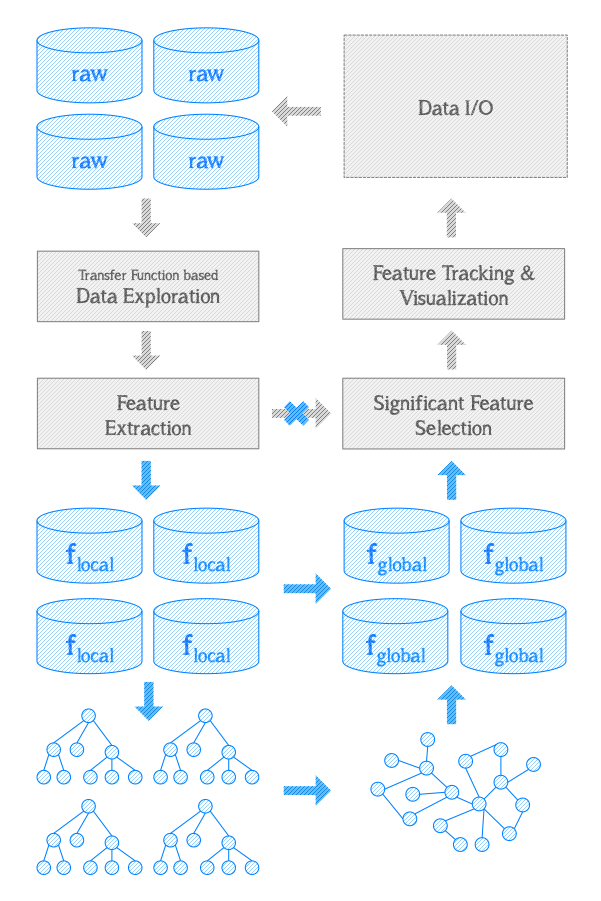
\includegraphics[width=1\linewidth]{system_overview.png}
	\caption{Work flow of a single time-step}
	\label{fig:system-overview}
\end{figure}

First, the source volume data is read either from a pre-generated data set or from a simulation program in-situ. Then, user can identify features of interest via transfer function manipulation as such candidate features will be extracted. However, since the descriptive power of a transfer function is often insufficient to precisely highlight the desired subset of features, user may have to select significant features either by simple point-and-select or iteratively filter out unwanted ones using different feature descriptors. Once the user has identified the interesting features, the system tracks only these significant features in subsequent time steps.

What our approach distinct from that of the previous one lies in that the global connectivity information of each feature need to be obtained before the Significant Feature Selection process could be carried out. As shown in blue color in Figure~\ref{fig:system-overview}, first the raw data are distributed in \textcolor{red}{logically adjacent data blocks.}. After Feature Extraction is done in each data block, the set of local features as well as the local connectivity information will be generated. Then by applying our merging algorithms, global connectivity information can be obtained efficiently such that each data block will possess the global connectivity information for each of its residing features. This enables Signification Feature Selection in a distributed environment and henceforth Feature Tracking and Visualization.